\documentclass[9pt,twocolumn,twoside]{../../styles/osajnl}
\usepackage{fancyvrb}
\journal{i524} 

\title{Google Dremel: SQL-Like Query for  Big Data}


\author[1,*]{Jimmy Ardiansyah}

\affil[1]{School of Informatics and Computing, Bloomington, IN 47408, U.S.A.}


\affil[*]{jardians@indiana.edu - S17-IR-2002}

\dates{Research Article-01, \today}

\ociscodes{Google Dremel, Big Data Query}

% replace this with your url in github/gitlab
\doi{\url{https://github.com/jardians/sp17-i524/tree/master/paper1/S17-IR-2002/report.pdf}}
 
\begin{abstract}
Dremel is a scalable, interactive ad-hoc query system for analysis of read-only nested data. By combining multi-level  execution trees and columnar data layout, it is capable of running aggregation queries over trillion-row tables in seconds.\newline  
\end{abstract} 

   
\setboolean{displaycopyright}{true} 

\begin{document}

\maketitle



\section{Introduction}
Big data analytics nowadays has become more common across industries and government agencies partly due to fast and affordable commodity storage to keep pace with data and business growth.  

Make the data sense at the fingertips of data scientists and analysts has become increasingly essential to compete in the business world. Having interactive tool with fast response times often make a difference in data exploration, rapid prototyping as well as designing of data pipelines. Performing interactive data analysis at scale demands a high degree of parallelism. That's where Dremel comes into play.

Dremel is a scalable, interactive ad-hoc query system for analysis of read-only nested data. By combining multi-level execution trees and columnar data layout, it is capable of running aggregation queries over trillion-row tables in seconds.  The system scales to thousands of CPUs and petabytes of data.  With Dremel, you get to write a declarative SQL-like query against data stored in a very efficient for analysis read-only columnar format. It's also possible to write queries that analyze billions of rows, terabytes of data, and trillions of records in seconds ~\cite{paper-dremel}. 

\section{History Development}
When Google published the Dremel paper in 2010, it explained how this structure is preserved within column store. Every column, in addition to its value, also stores two numbers — definition and repetition levels.

This encoding ensures that the full or partial structure of the record can be reconstructed by reading only requested columns, and never requires reading parent columns (which is the case with alternative encoding). That same paper gives an exact algorithm for both encoding the data and reconstructing the record.

In 2014, Google published another paper — Storing and Querying tree-structured records in Dremel ~\cite{www-dremel}  — which lays theoretical foundation and proves correctness of algorithms for filtering and aggregation operators, which take advantage of the above encoding.

\section{Design}

Dremel supports interactive analysis of very large datasets over shared clusters of commodity machines.  Dremel can even execute a complex regular expression text matching on a huge logging table in merely tens of seconds. This is the power of Dremel; it has high scalability and most of the time it returns results within seconds or tens of seconds no matter how big the queried dataset is. These two core technologies gives Dremel high performance in analyzing large datasets: 

\begin{enumerate}
  \item 	Columnar Storage. Data is stored in a columnar storage fashion which makes possible to achieve  high compression ratio and scan throughput.
  \item Tree Architecture is used for dispatching queries and aggregating results across thousands of machines. ~\cite{paper-dremel}.
\end{enumerate}

\subsection{Columnar Storage.}
Dremel stores data in its columnar storage, which means it separates a record into column values and stores each value on different storage volume, whereas traditional databases normally store the whole record on one volume; this is efficient for cases where many columns of the records need to be fetched. For example, if one analysis heavily relied on fetching all fields for records that belong to a particular time ranged, row-oriented storage would make sense. 

To illustrate what columnar storage is all about, here is an example with three columns in the Figure-1


\begin{figure}[H]
 \centering
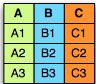
\includegraphics[scale=0.7]{images/image1}
\caption{Typical row-oriented storage}
\end{figure}



In a row-oriented storage, the data is laid out one row at a time as follows in the Figure-2:


\begin{figure}[H]
 \centering
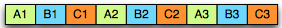
\includegraphics[scale=0.7]{images/image2}
\caption{Transform row to column-oriented format}
\end{figure}

Whereas in a column-oriented storage, it is laid out one column at a time in the Figure-3:

\begin{figure}[H]
 \centering
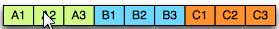
\includegraphics[scale=0.7]{images/image3}
\caption{Laid out the column}
\end{figure}

Dremel has introduced columnar storage, which  provides several advantages over row-oriented system:

\begin{itemize}
  \item it is generally efficient in term of compression on columns because entropy within a column is lower that entropy within a block of rows. in other words, data is more similar within the same column, than it is in a block of rows. This can make a big difference especially when the column has few distinct values.
  \item Work well for queries that only access a small subset of columns. 
  \item I/O will be reduced as we can efficiently scan only a subset of the columns while reading the data. Better compression also reduces the bandwidth required to read the input.
  \item Is often well suited for data-werehousing applications where users want to aggregate certain columns over a large collection of records. 
  \item As we store data of the same type in each column, we can use encoding better suited to the modern processors’ pipeline by making instruction branching more predictable ~\cite{book-hadoop-apps}.
\end{itemize}


\subsection{Tree Architecture}
Dremel builds on ideas from web search and parallel DBMSs. First, its architecture borrows the concept of a serving tree used in distributed search engines. Figure- 4 shows a serving three execution model. Just like a web search request, a query gets pushed down the tree and is rewritten at each step. The result of the query is assembled by aggregating the replies received from lower levels of the tree. Tree Architecture has enable Dremel to dispatch queries and collect results across tens of thousands of machines in a matter of seconds by using the Tree architecture ~\cite{book2-hadoop}. The architecture forms a massively parallel distributed tree for pushing down a query to the tree and then aggregating the results from the leaves at a fast speed ~\cite{twitter-dremel}. Consider a simple aggregation query below:

\begin{figure}[H]
 \centering
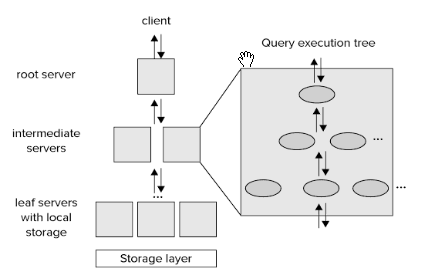
\includegraphics[scale=0.7]{images/image4}
\caption{Typical Tree Architecture ~\cite{book-hadoop}} 
\end{figure}

A root server receives incoming queries, reads metadata from the tables, and routes the queries to the next level intermediate servers in the serving tree. The leaf servers communicate with the storage layer (based on the columnar model described earlier) to read data which is bubbling up for the aggregation and final result is return to the user  or access the data on local disk. 

However, after data is processed, one will be running aggregate queries and analysis on large chunks of data at a time, most probably only on a subsets of columns. Because many analytical queries only select a subsets of columns at a time for storing that will be analyzed later ~\cite{book-hadoop}.

Overall, Dremel combines parallel query execution with the columnar format that supporting  performance data access and also capable of operating on in place nested data. In place refers to the ability to process and analyze large, fast-moving datasets where it resides e.g., in a distributed file system like Veritas Cluster File System,  General Parallel File System (GPFS), and  Global File System (GFS). 

\section{Implementation of Google Dremel }
Apache Drill is the open source version of Google's Dremel system which is available as an infrastructure service called Google BigQuery ~\cite{wiki-radar}. One explicitly stated design goal is that Drill is able to scale to 10,000 servers or more and to be able to process petabytes of data and trillions of records in seconds~\cite{wiki-drill}. Drill is an Apache top-level project. Open source project must pass Apache incubator process which is the gateway for open source project intended to become top-level or fully fledged Apache Software Foundation (ASF) projects.  Drill supports a variety of NoSQL databases and file systems. In addition, Drill supports data locality, so it's a good idea to co-locate Drill and the datastore on the same nodes.

\section{Conclusion}
 Although query and process large volume of data in any system are a challenging task, especially in the big data ecosystem due to vast expense of option available, Dremel has shown as the right model for process and storing data with a lot of benefits as well as fitting as part of an entire big data stack which can be used against raw data, like log data.  Choosing the right tool for your data is one of the most important decision one will make in the application, and everyone need to spend the appropriate amount of time and effort to get it right the first time. Because of it,  Dremel's design could be the future of interactive ad-hoc query system for analysis that require fast result. 
 
 \section{Acknowledgements}
this work was done as part of the course "I524: Big Data and Open Source Software Projects" at Indiana University during Spring 2017


% Bibliography

\bibliography{references}
 
\end{document}

